\documentclass[border=0pt]{standalone}
\usepackage{tikz}
\usetikzlibrary{decorations.pathreplacing,
  arrows,
  calc,
  decorations.pathmorphing,
  decorations.pathreplacing,
  decorations.markings,
  fadings,
  positioning,
  shapes,
  3d
}
\tikzfading[name=fade img right,left color=transparent!100, right color=transparent!0]
\tikzfading[name=fade img left,right color=transparent!100, left color=transparent!0]
\tikzstyle{snakearrow} = [decorate, decoration={pre length=0.1cm,
  post length=0.1cm, snake, amplitude=.4mm,
  segment length=4mm},thick, ->]
\usepackage{graphicx}
\begin{document}
\newcommand*{\arrowthreeD}[5]{%
  \fill[left color=#1!50!black,right color=#1!50!black,middle color=#1!43,
  opacity=0.9,
  transform canvas={shift={#2}, rotate=#3},shading=axis,shading angle=90]
  (0,0) -- (80:#4) arc (80:100:#4) -- cycle;
  \fill[left color=#1!50!black,right color=#1!50!black,middle color=#1!43,
  opacity=0.9,
  transform canvas={shift={#2}, rotate=#3},shading=axis,shading angle=90]
  (87:#4) -- ++(0, #5) -- ++(-{2 * #4 * sin(3)}, 0) -- (93:#4) -- cycle;
}
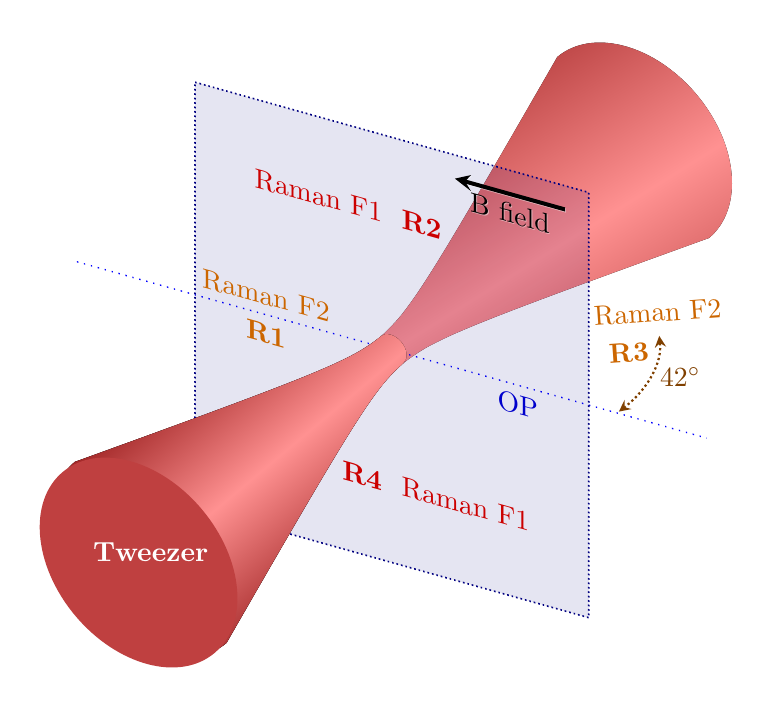
\begin{tikzpicture}
  \pgfmathsetmacro{\radiush}{1.5}
  \pgfmathsetmacro{\theight}{4}
  \pgfmathsetmacro{\radiusv}{.7 * \radiush}
  \pgfmathsetmacro{\waist}{.15}
  \pgfmathsetmacro{\xscale}{\radiush / sqrt(1 + (\waist)^2)}

  \fill[left color=red!50!black,right color=red!50!black,middle color=red!43,
  shading=axis,rotate=-50,shading angle=32]
  plot[domain={-1}:{1}, smooth, variable=\y] ({sqrt((\y)^2 + (\waist)^2) * \xscale}, \y * \theight)
  arc (0:180:\radiush cm and \radiusv cm)
  -- plot[domain={-1}:{1}, smooth, variable=\y] ({-sqrt((\y)^2 + (\waist)^2) * \xscale}, -\y * \theight)
  arc (180:360:\radiush cm and \radiusv cm);

  \begin{scope}[transform canvas={rotate={4}}]
    \arrowthreeD{orange}{(0.6, 0)}{-90}{0.4}{3.2};
    \path (3.4, 0) node[above,orange!80!black] {Raman F2};
    \path (3, 0) node[below,orange!80!black] {\textbf{R3}};
  \end{scope}

  \draw[orange!50!black, <->, densely dotted, >=stealth, line width=0.8]
  (3:3.4) arc (3:-32:3.4 and 1.65);
  \path (-6:3.3) node[orange!50!black, right] {$42^\circ$};

  \begin{scope}[transform canvas={cm={1,-0.28,0,1,(0, 0)}}]
    \draw[blue, dotted, line width=0.5] (-4.0, 0) -- (4.0, 0);

    \fill[blue!50!black,opacity=0.1] (-2.5, 2.7) -- (2.5, 2.7)
    -- (2.5, -2.7) -- (-2.5, -2.7) -- cycle;
    \draw[blue!50!black, densely dotted,line width=0.6] (-2.5, 2.7) -- (2.5, 2.7)
    -- (2.5, -2.7) -- (-2.5, -2.7) -- cycle;
    \arrowthreeD{red}{(0, -0.4)}{180}{0.4}{1.4};
    \arrowthreeD{orange}{(-0.4, 0)}{90}{0.4}{1.4};
    \arrowthreeD{blue}{(0.4, 0)}{-90}{0.4}{1.4};
    \arrowthreeD{red}{(0, 0.4)}{0}{0.4}{1.4};
    \path (1.6, 0) node[below,blue!80!black] {OP};
    \path (-1.6, 0) node[above,orange!80!black] {Raman F2};
    \path (-1.6, 0) node[below,orange!80!black] {\textbf{R1}};

    \path (0, 1.7) node[left,red!80!black] {Raman F1};
    \path (0, 1.7) node[right,red!80!black] {\textbf{R2}};

    \path (0, -1.7) node[left,red!80!black] {\textbf{R4}};
    \path (0, -1.7) node[right,red!80!black] {Raman F1};

    \draw[white,opacity=0.5,->,>=stealth,line width=1.5] (2.21, 2.39) -- (0.81, 2.39);
    \draw[->,>=stealth,line width=1.5] (2.2, 2.4) -- (0.8, 2.4);
    \path (1.51, 2.39) node[below,white,opacity=0.5] {B field};
    \path (1.5, 2.4) node[below] {B field};
  \end{scope}

  \fill[left color=red!50!black,right color=red!50!black,middle color=red!43,
  shading=axis,rotate=-50,shading angle=40]
  plot[domain={-1}:{0}, smooth, variable=\y] ({sqrt((\y)^2 + (\waist)^2) * \xscale}, \y * \theight)
  arc (0:180:{(\radiush)*(\waist)} and {(\radiusv)*(\waist)})
  -- plot[domain={0}:{1}, smooth, variable=\y] ({-sqrt((\y)^2 + (\waist)^2) * \xscale}, -\y * \theight)
  arc (180:360:\radiush cm and \radiusv cm);
  \fill[red!50!gray,rotate=-50]
  ({-sqrt(1 + (\waist)^2) * \xscale}, -\theight*1.05)
  arc (180:{360+180}:\radiush cm and \radiusv cm);

  \path (-140:\theight) node[white] {\textbf{Tweezer}};
\end{tikzpicture}

\end{document}
